\section{Mage's Ballad}

Although Mage's Ballad is usually the second song played in a song sequence, it is the simplest song to handle how Repertoire procs leads to additional ability usages. Under the effect of Mage's Ballad, each Repertoire proc will shorten the recast time of Heartbreak Shot and Rain of Death by 7.5s, half of total recast time. A single target encounter where Heartbreak Shot (HS) is used is assumed. Immediate usage of HS procs is also assumed. Since two Repertoire procs are required for one HS usage, achieving $k_{hs}$ HS procs due to $k_r$ Repertoire procs is given by

\begin{equation}
    k_{hs} = \lceil k_{r} / 2 \rceil
\end{equation}

Where $\lceil \cdot \rceil$ denotes a ceiling operation. The ceiling operator accounts for the fact that an odd number of Repertoire procs still grants the maximum possible number of HS usages due to the guaranteed Repertoire proc from Empyreal Arrow.\footnote{This is a simplification for HS accounting purposes. Realistic 3-6-9 song sequences require more careful accounting.} The probability of attaining $k_{hs}$ HS usages due to Repertoire procs is

\begin{equation}
    P_{hs}(k_{hs}; n_r, p_r) = \sum_{j=\max(0, 2k_{hs}-1)}^{2k_{hs}} P_r(k_r = j; n_r)
\end{equation}


The HS proc distribution for a full 45s Mage's Ballad with 15 Repertoire ticks is shown below, Figure \ref{fig:hs-proc-distribution}.

\begin{figure}[H]
    \centering
    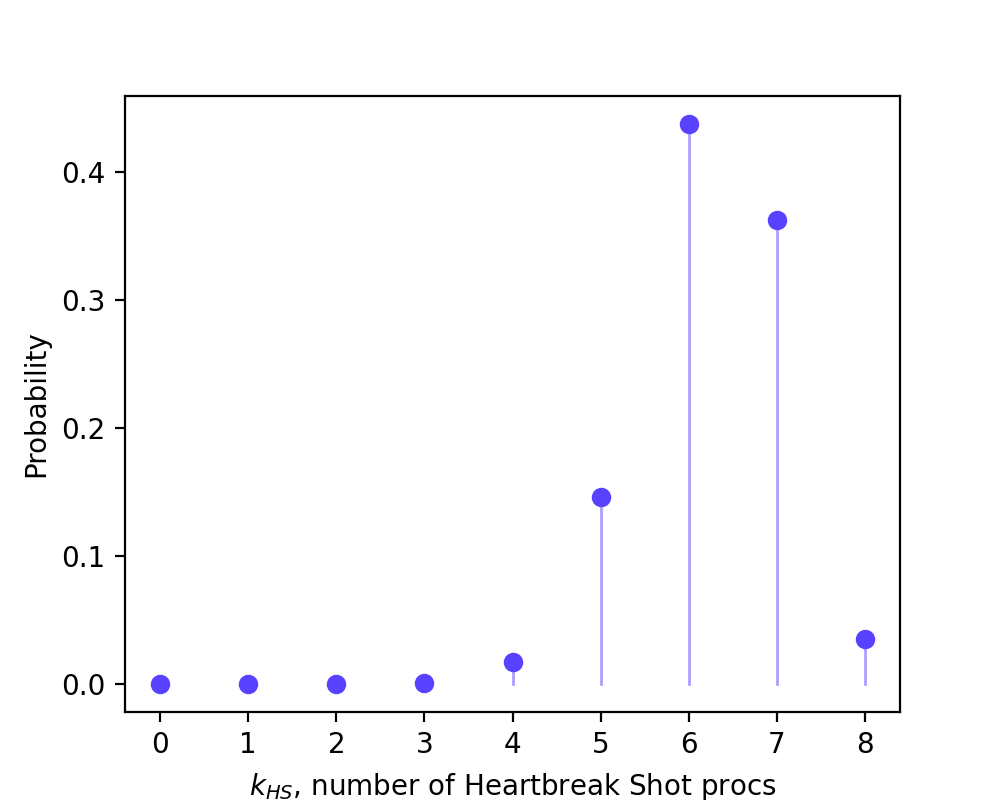
\includegraphics[scale=0.65]{img/hs-proc-distribution.png}
    \caption{Heartbreak Shot proc count probability distribution for the full duration of Mage's Ballad.}
    \label{fig:hs-proc-distribution}
\end{figure}

Due to the relative simplicity of proc usage and lack of multiple buff windows to consider, we can exactly account for HS proc variability for a full uptime encounter. The damage distribution will be a mixture distribution of all possible HS proc counts,

\begin{equation}
    P(D_{hs}) = \sum_{k_{hs}=0}^8 P_{hs}(k_{hs}) P(D_{hs}; n_{hs} = k_{hs})
\end{equation}

Recall sase damage values and combat simulation parameters can be found in Table \ref{t:combat-params}. Only the 1\% damage buff from Mage's Ballad is applied. These parameters are used to compute the damage distribution for HS procs due to Repertoire procs. In addition, the damage distribution for the most probable number of HS procs, $k_{hs} = 6$ is also computed to compare the effects of assuming the most likely HS proc rate, Figure \ref{fig:hs-dmg-distribution}.

\begin{figure}[H]
    \centering
    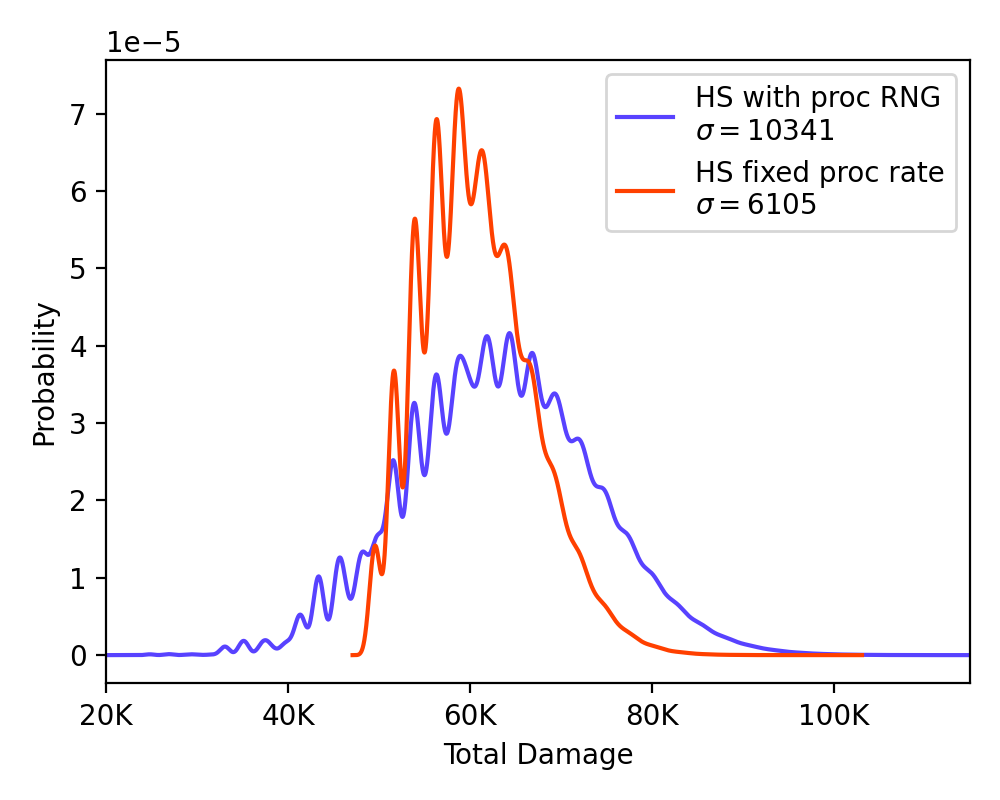
\includegraphics[scale=0.65]{img/hs-dmg-distribution.png}
    \caption{Damage distribution of Heartbreak Shot procs under Mage's Ballad (blue) and Heartbreak Shot damage distribution assuming an average proc rate (orange).}
    \label{fig:hs-dmg-distribution}
\end{figure}

The standard deviation when accounting for HS proc variability increases by a substantial 69\%. While the increase is large and suggests proc variability may be important, the total damage dealt by HS procs relative to all of Bard's damage output is $< 10\%$ of Bard's overall damage.